% !TeX encoding = UTF-8
% !TeX spellcheck = pl_PL

% $Id:$

%Author: Wojciech Domski
%Szablon do ząłożeń projektowych, raportu i dokumentacji z steorwników robotów
%Wersja v.1.0.0
%

%% Konfiguracja:
\newcommand{\kurs}{Sterowniki robot\'{o}w}
\newcommand{\formakursu}{Projekt}

%odkomentuj właściwy typ projektu, a pozostałe zostaw zakomentowane
%\newcommand{\doctype}{Za\l{}o\.{z}enia projektowe} %etap I
\newcommand{\doctype}{Raport} %etap II
%\newcommand{\doctype}{Dokumentacja} %etap III

%wpisz nazwę projektu
\newcommand{\projectname}{Automatyczny barman Dionizos}

%wpisz akronim projektu
\newcommand{\acronim}{AuBaDi}

%wpisz Imię i nazwisko oraz numer albumu
\newcommand{\osobaA}{Kewin \textsc{Gałuszka}, 241624}
\newcommand{\osobaB}{Adrian \textsc{Urban}, 241558}
%w przypadku projektu jednoosobowego usuń zawartość nowej komendy


%wpisz termin w formie, jak poniżej dzień, parzystość, godzina
\newcommand{\termin}{ptTP11}

%wpisz imię i nazwisko prowadzącego
\newcommand{\prowadzacy}{dr in\.{z}. Wojciech \textsc{Domski}}

\documentclass[10pt, a4paper]{article}
\usepackage{float}
\usepackage{polski}
\usepackage{breakurl}
\usepackage[hyphens]{url}
\usepackage{hyperref}
\usepackage[utf8]{inputenc}
\usepackage{lscape}
\usepackage{pdfpages}
\usepackage{url}

%Preambuła dokumentu

% linki w spisie tresci, bibliografi
\usepackage[bookmarks=true,bookmarksnumbered=false,unicode=true,pdftex=true, colorlinks,filecolor=black,linkcolor=black,urlcolor=black,citecolor=black]{hyperref}

%ustawienie rozmiaru papieru
\usepackage[a4paper, left=2.5cm, right=2.5cm, top=2.5cm, bottom=2.5cm, headsep=1.2cm]{geometry}

%rozmaite ustawienia pozwalające okreslić język

%NALEŻY wybrać jeden z pakietów
%\usepackage{polski} %przydatne podczas składania dokumentów w j. polskim
\usepackage[polish]{babel}  % pakiet lokalizujący dokument w języku polskim
%\usepackage[british]{babel}

\usepackage{indentfirst}	% polski styl pisania (np. rozpoczecie pierwszego akapitu
% pod nazwa rozdzialu od wciecia)
%\usepackage[OT4]{fontenc}
\usepackage[utf8]{inputenc} % w miejsce utf8 można wpisać latin2 bądź cp1250,
% w zależności od tego w jaki sposób kodowane są 
% polskie znaki diakrytyczne przy wprowadzaniu 
% z klawiatury.
%kodowanie znaków, zależne od systemu
\usepackage[T1]{fontenc} %poprawne składanie polskich czcionek

%OPEROWANIE NA OBRAZACH
\usepackage{graphicx}       % pakiet graficzny, umożliwiający m.in.
% import grafik w formacie eps
%\usepackage{epstopdf}		% pozwala na importowanie grafik w formacie eps
% przy użyciu pdflatex
\usepackage[update,prepend]{epstopdf}
\usepackage{rotating}       % pakiet umożliwiający obracanie rysunków
\usepackage{subfigure}      % pakiet umożliwiający tworzenie podrysunków
\usepackage{epic}           % pakiet umożliwiający rysowanie w środowisku latex
\usepackage{psfrag}         % pakiet umożliwiający podmianę łańcuchów znaków 
% w plikach eps
%\usepackage{curves}         % pakiet do wykreslania krzywych

%pakiety dodające dużo dodatkowych poleceń matematycznych
\usepackage{amsfonts}       % pakiet z rozmaitymi czcionkami matematycznymi
%\usepackage{amssymb}        % pakiet z rozmaitymi symbolami matematycznymi
\usepackage{amsmath}        % pakiet z rozmaitymi środowiskami matematycznymi

\usepackage{fp}             % pakiet z funkcjami operujacymi 
% na liczbach zmiennoprzecinkowych
\usepackage{calc}           % pakiet umożliwiający operacje arytmetyczne
% na tzw. licznikach (liczbach całkowitych)
\usepackage{leftidx}		% indeksy górne i dolne po lewej stronie

%definicje matematyczne
\providecommand{\abs}[1]{\lvert#1\rvert}
\providecommand{\norm}[1]{\lVert#1\rVert}

%pakiety wspomagające i poprawiające składanie tabel
\usepackage{supertabular}
\usepackage{array}
\usepackage{tabularx}
\usepackage{hhline}
\usepackage{longtable}		% wsparcie dla dlugich tabel
\usepackage{multicol}		% podzial strony na wiele kolumn

%pakiet do BibTex
\usepackage{cite}

\usepackage{url} %pakiet pozawalający na dodawanie adresów url w bibliografi

%pakiet wypisujący na marginesie etykiety równań i rysunków zdefiniowanych przez \label{}, chcąc wygenerować finalną wersję dokumentu wystarczy usunąć poniższą linię
%\usepackage{showlabels}

\usepackage{float}			% lepsza obsluga mechanizmow obiektow plywajacych
% wymuszenie wstawienia np. tabeli, obrazka w danym miejscu przez [H]

\usepackage{listings}       % pakiet dedykowany zrodlom programow
\usepackage{color}


\definecolor{dkgreen}{rgb}{0,0.6,0}
\definecolor{gray}{rgb}{0.5,0.5,0.5}
\definecolor{mauve}{rgb}{0.58,0,0.82}

\lstset{ %
	language=C,                % the language of the code
	basicstyle=\small,           % the size of the fonts that are used for the code
	numbers=left,                   % where to put the line-numbers
	numberstyle=\footnotesize\color{gray},  % the style that is used for the line-numbers
	stepnumber=1,                   % the step between two line-numbers. If it's 1, each line 
	% will be numbered
	numbersep=5pt,                  % how far the line-numbers are from the code
	backgroundcolor=\color{white},      % choose the background color. You must add \usepackage{color}
	showspaces=false,               % show spaces adding particular underscores
	showstringspaces=false,         % underline spaces within strings
	showtabs=false,                 % show tabs within strings adding particular underscores
	%frame=single,                   % adds a frame around the code
	rulecolor=\color{black},        % if not set, the frame-color may be changed on line-breaks within not-black text (e.g. comments (green here))
	tabsize=2,                      % sets default tabsize to 2 spaces
	captionpos=b,                   % sets the caption-position to bottom
	breaklines=true,                % sets automatic line breaking
	breakatwhitespace=false,        % sets if automatic breaks should only happen at whitespace
	%title=\lstname,                   % show the filename of files included with \lstinputlisting;
	% also try caption instead of title
	keywordstyle=\color{blue},          % keyword style
	commentstyle=\color{dkgreen},       % comment style
	stringstyle=\color{mauve},         % string literal style
	escapeinside={\%*}{*)},            % if you want to add LaTeX within your code
	morekeywords={*,...},              % if you want to add more keywords to the set
	deletekeywords={...}              % if you want to delete keywords from the given language
}

%polish signs in lst code
\lstset{literate=%
	{ą}{{\k{a}}}1
	{ć}{{\'c}}1
	{ę}{{\k{e}}}1
	{ł}{{\l}}1
	{ń}{{\'n}}1
	{ó}{{\'o}}1
	{ś}{{\'s}}1
	{ż}{{\.z}}1
	{ź}{{\'z}}1
	{Ą}{{\k{A}}}1
	{Ć}{{\'C}}1
	{Ę}{{\k{E}}}1
	{Ł}{{\L}}1
	{Ń}{{\'N}}1
	{Ó}{{\'O}}1
	{Ś}{{\'S}}1
	{Ż}{{\.Z}}1
	{Ź}{{\'Z}}1
}

\usepackage{verbatim}       % pakiet dedykowany rozmaitym wydrukom tekstowym
\usepackage{ifthen}         % pakiet umożliwiający tworzenie prostych programów
% (m.in. zawiera instrukcje powtórzeniowe 
% i warunkowe)
\usepackage{upquote}		%normal quotations marks ' and `

% deklaracje wymagane przez pakiet theorem automatycznie ladowany w przypadku
% klasy dokumentu article
%
\newtheorem{Dn}{Definicja}[section]     % deklaracja srodowiska definicja
\newtheorem{La}[Dn]{Lemat}                % deklaracja srodowiska lemat
\newtheorem{Tm}[Dn]{Twierdzenie}          % deklaracja srodowiska twierdzenie
\newtheorem{Rk}[Dn]{Spostrze{\.z}enie}  % deklaracja srodowiska spostrzezenie
\newtheorem{Am}[Dn]{Algorytm}           % deklaracja srodowiska algorytm
\newtheorem{As}[Dn]{Za{\l}o{\.z}enie}   % deklaracja srodowiska zalozenie
\newtheorem{Pn}[Dn]{Propozycja}           % deklaracja srodowiska propozycja
\newtheorem{Py}[Dn]{W{\l}asno{\'s}{\'c}}  % deklaracja srodowiska wlasnosc
\newtheorem{Cy}[Dn]{Wniosek}              % deklaracja srodowiska wniosek
\newtheorem{Ee}[Dn]{Przyk{\l}ad}        % deklaracja srodowiska przyklad
\newtheorem{Ex}{{\'C}wiczenie}          % deklaracja srodowiska cwiczenie

%helps to specify width of a column in table
%\begin{tabular}{|C{1cm}|c|c|c|c|c|c|c|c|c|c|}
%first column will have widht of 1cm
\newcolumntype{L}[1]{>{\raggedright\let\newline\\\arraybackslash\hspace{0pt}}m{#1}}
\newcolumntype{C}[1]{>{\centering\let\newline\\\arraybackslash\hspace{0pt}}m{#1}}
\newcolumntype{R}[1]{>{\raggedleft\let\newline\\\arraybackslash\hspace{0pt}}m{#1}}

\sloppy			%zawija bardzo długie linie

%\pagenumbering{gobble}% Remove page numbers (and reset to 1)

\begin{document}

\def\tablename{Tabela}	%zmienienie nazwy tabel z Tablica na Tabela

\begin{titlepage}
	\begin{center}
		\textsc{\LARGE \formakursu}\\[1cm]		
		\textsc{\Large \kurs}\\[0.5cm]		
		\rule{\textwidth}{0.08cm}\\[0.4cm]
		{\huge \bfseries \doctype}\\[1cm]
		{\huge \bfseries \projectname}\\[0.5cm]
		{\huge \bfseries \acronim}\\[0.4cm]
		\rule{\textwidth}{0.08cm}\\[1cm]
		
		\begin{flushright} \large
		\emph{Skład grupy:}\\
		\osobaA\\
		\osobaB\\[0.4cm]
		
		\emph{Termin: }\termin\\[0.4cm]

		\emph{Prowadzący:} \\
		\prowadzacy \\
		
		\end{flushright}
		
		\vfill
		
		{\large \today}
	\end{center}	
\end{titlepage}

\newpage
\tableofcontents
\newpage

%Obecne we wszystkich dokumentach
\section{Opis projektu}
\label{sec:OpisProjektu}

Celem projektu jest stworzenie automatycznego barmana -- urządzenia będącego w stanie mieszać płyny w ściśle zadanych proporcjach. Urządzenie wyposażone w wyświetlacz LCD oraz przyciski będzie oferować interfejs, który pozwoli użytkownikowi na wybranie konkretnego napoju. W zależności od decyzji użytkownika dotyczącej rodzaju napoju, urządzenie zmieni swoje podświetlenie wykonane za pomocą diod LED. Dodatkowo wykorzystany zostanie DAC do wygenerowania wcześniej zapisanego na pamięć dźwięku. Karetka, w której umieszczony zostanie zbiornik na płyn będzie przesuwana za pomocą silnika krokowego. Kolejne płyny będą pobierane z zasobników za pomocą indywidualnych pomp bądź zaworów.

\begin{figure}[H]
	\centering
	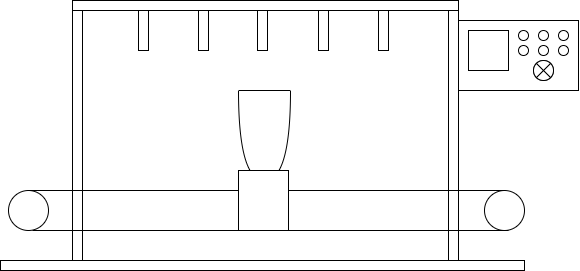
\includegraphics[width=0.7\textwidth]{figures/dionizos.png}
	\caption{Schematyczny rysunek urządzenia}
	\label{fig:Architektura}
\end{figure}

%Obecne we wszystkich dokumentach
\section{Konfiguracja mikrokontrolera}
 
Konfiguracja portów mikrokontrolera (rysunek 2) oraz zegarów (rysunek 3) przy użyciu prgoramu STM32CubeMX.
 
\begin{figure}[H]
	\centering
	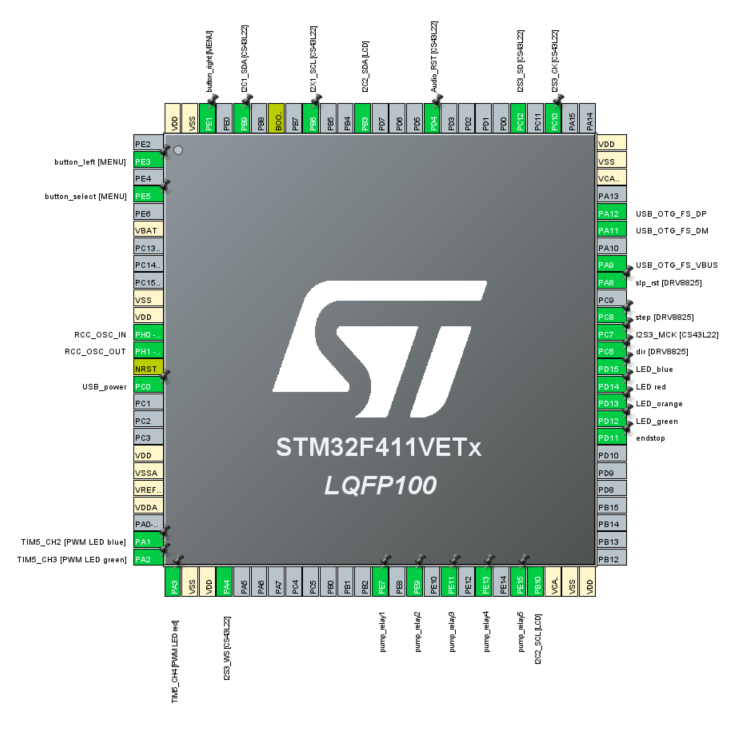
\includegraphics[width=0.6\textwidth]{nowa_konfiguracja.PNG}
	\caption{Konfiguracja wyjść mikrokontrolera w programie STM32CubeMX}
	\label{fig:KonfiguracjaMikrokontrolera}
\end{figure}

\newpage
\begin{figure}[H]
	\centering
	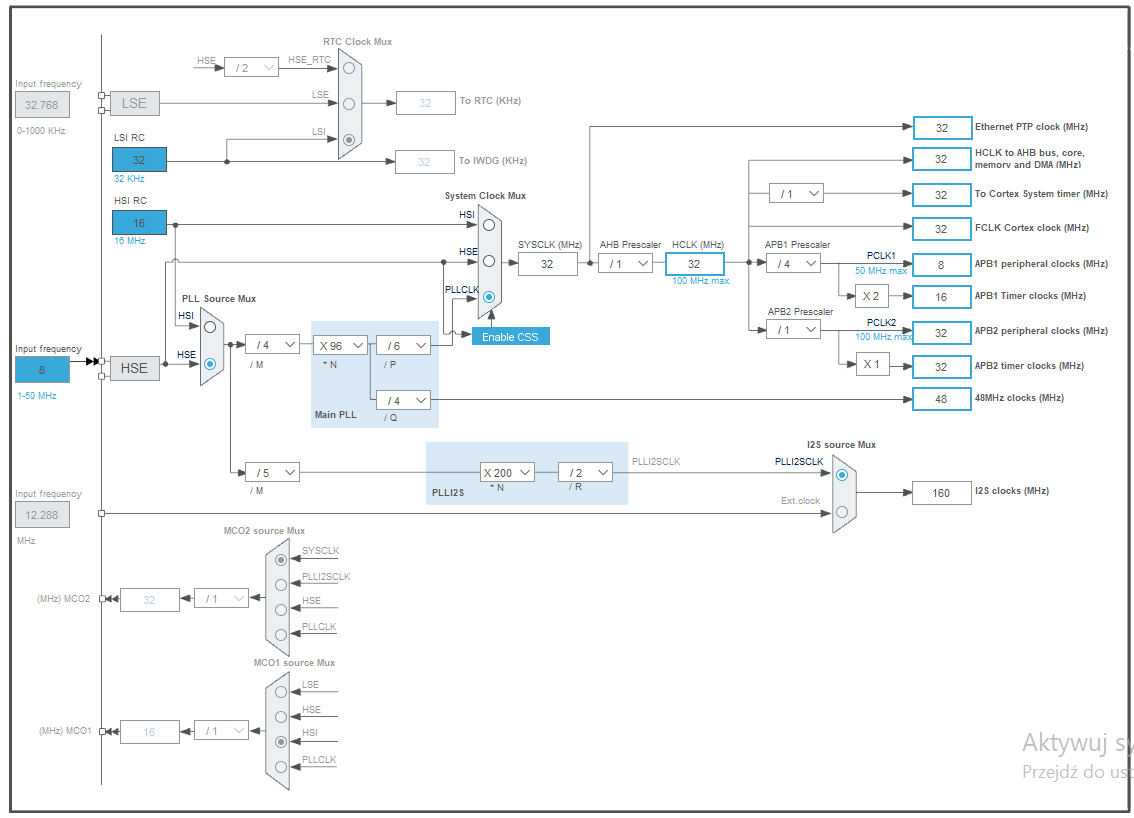
\includegraphics[width=0.9\textheight,angle=90]{zegary.PNG}
	\caption{Konfiguracja zegarów mikrokontrolera}
	\label{fig:KonfiguracjaZegara}
\end{figure}

%Obecne we wszystkich dokumentach
\subsection{Konfiguracja pinów}

\begin{table}[H]
	\centering
	\begin{tabular}{|l|l|l|l|}
		\hline
		Numer pinu	&	PIN & Tryb pracy & Funkcja/etykieta\\
		\hline
2&	PE3&	GPIO{\_}EXTI3&	button{\_}left [MENU] \\
4&	PE5&	GPIO{\_}EXTI5&	button{\_}select [MENU] \\
12&	PH0 - OSC{\_}IN&	RCC{\_}OSC{\_}IN& --	\\
13&	PH1 - OSC{\_}OUT&	RCC{\_}OSC{\_}OUT& --\\
15&	PC0&	GPIO{\_}Output&	USB{\_}power\\
24&	PA1&	TIM5{\_}CH2&	TIM5{\_}CH2 [PWM LED blue] \\
25&	PA2&	TIM5{\_}CH3&	TIM5{\_}CH3 [PWM LED green] \\
26&	PA3&	TIM5{\_}CH4&	TIM5{\_}CH4 [PWM LED red] \\
29&	PA4&	I2S3{\_}WS&	I2S3{\_}WS [CS43L22] \\
38&	PE7&	GPIO{\_}Output&	pump{\_}relay1\\
40&	PE9&	GPIO{\_}Output& pump{\_}relay2\\
42&	PE11&	GPIO{\_}Output&	pump{\_}relay3\\
44&	PE13&  GPIO{\_}Output&	pump{\_}relay4\\
46&	PE15&	GPIO{\_}Output& pump{\_}relay5\\
47&	PB10&	I2C2{\_}SCL&	I2C2{\_}SCL [LCD] \\
58&	PD11&	GPIO{\_}EXTI11&	endstop\\
59&	PD12&	GPIO{\_}Output&	LED{\_}green\\
60&	PD13&	GPIO{\_}Output&	LED{\_}orange\\
61&	PD14&	GPIO{\_}Output&	LED red\\
62&	PD15&	GPIO{\_}Output&	LED{\_}blue\\
63&	PC6&	GPIO{\_}Output&	dir [DRV8825] \\
64&	PC7&	I2S3{\_}MCK&	I2S3{\_}MCK [CS43L22] \\
65&	PC8&	GPIO{\_}Output&	step [DRV8825] \\
67&	PA8&	GPIO{\_}Output&	slp{\_}rst [DRV8825] \\
68&	PA9&	USB{\_}OTG{\_}FS{\_}VBUS&--	 \\
70&	PA11&	USB{\_}OTG{\_}FS{\_}DM& --\\	
71&	PA12&  USB{\_}OTG{\_}FS{\_}DP&--	 \\
78&	PC10&	I2S3{\_}CK& 	I2S3{\_}CK [CS43L22] \\
80&	PC12&	I2S3{\_}SD&	I2S3{\_}SD [CS43L22] \\
85&	PD4&	GPIO{\_}Output&	Audio{\_}RST [CS43L22] \\
89&	PB3&	I2C2{\_}SDA&	I2C2{\_}SDA [LCD] \\
92&	PB6&	I2C1{\_}SCL&	I2C1{\_}SCL [CS43L22] \\
96&	PB9&	I2C1{\_}SDA&	I2C1{\_}SDA [CS43L22] \\
98&	PE1&	GPIO{\_}EXTI1&	button{\_}right [MENU] \\


		\hline
	\end{tabular}
	\caption{Konfiguracja pinów mikrokontrolera}
	
\end{table}
\begin{itemize}
\item Piny PE7,PE9,PE11,PE13,PE15 -- załączanie przekaźników pomp
\item Piny PB6 i PB9 -- komunikacja I2C z DAC Audio
\item Piny PA4, PC7, PC10, PC12 -- komunikacja I2S z DAC Audio
\item Pin PD4 -- Reset DAC Audio
\item Piny PA1, PA2, PA3 -- oświetlenie LED
\item Piny PE1, PE3, PA5 -- przyciski
\item Piny PC6, PC8, PA8 -- sterownik silnika krokowego A4988
\item Piny PH0, PH1 -- rezonator kwarcowy
\item Pin PD11 -- wyłącznik krańcowy
\item Piny PB10, PB3 -- komunikacja I2C z wyświetlaczem LCD
\item Piny PA9, PA11, PA12, PD5 -- USB OTG (host)
\item Pin PC0 -- Zasilanie USB
\end{itemize}



%Obecne we wszystkich dokumentach
\subsection{I2C1}

Magistrala szeregowa I2C1 zostanie wykorzystana do komunikacji z układem CS43L22 -- DAC Audio

\begin{table}[H]
	\centering
	\begin{tabular}{|l|c|} \hline
		\textbf{Parametr} & Wartość \\
		\hline
		\hline  \textbf{I2C Speed Mode}& Standard Mode \\  \hline
		\textbf{I2C Clock Speed (Hz) } & 100000 \\
		
		\hline  \textbf{Primary Address Length selection}& 7-bit  \\\hline

	\end{tabular}
	\caption{Konfiguracja peryferium I2C1}
	\label{tab:USART}
\end{table}
\subsection{I2C2}

Magistrala szeregowa I2C2 zostanie wykorzystana do komunikacji z kontrolerem wyświetlacza HD44780 

\begin{table}[H]
	\centering
	\begin{tabular}{|l|c|} \hline
		\textbf{Parametr} & Wartość \\
		\hline
		\hline  \textbf{I2C Speed Mode}& Standard Mode \\  \hline
		\textbf{I2C Clock Speed (Hz) } & 100000 \\
		
		\hline  \textbf{Primary Address Length selection}& 7-bit  \\\hline

	\end{tabular}
	\caption{Konfiguracja peryferium I2C2}
	\label{tab:USART}
\end{table}
\subsection{I2S3}

Magistrala szeregowa I2S3 zostanie wykorzystana do komunikacji z układem CS43L22 -- DAC Audio 

\begin{table}[H]
	\centering
	\begin{tabular}{|l|c|} \hline
		\textbf{Parametr} & Wartość \\
		\hline
		\hline  \textbf{Transmission Mode}& Mode Master Transmit \\ 
		\hline  \textbf{Communication Standard} & I2S Philips \\
		\hline  \textbf{Data and Frame Format} & I2S 16 Bits Data on 16 Bits Frame \\
		\hline  \textbf{Selected Audio Frequency} & \textcolor{blue}{48KHz }\\
		\hline  \textbf{Real Audio Frequency} & \textcolor{blue}{48.076KHz} \\
		\hline  \textbf{Error between Selected and Real} & \textcolor{blue}{0.15{\%}}
		\\
	\hline  \textbf{Clock Source} & I2S PLL Clock  \\
	\hline  \textbf{Clock Polarity} & Low \\
	\hline

	\end{tabular}
	\caption{Konfiguracja peryferium I2S3}
	\label{tab:USART}
\end{table}



\subsection{USB OTG}

USB OTG zostanie wykorzystane do podłączenia zewnętrznej pamięci flash

\begin{table}[H]
	\centering
	\begin{tabular}{|l|c|} \hline
		\textbf{Parametr} & Wartość \\
		\hline
\hline  \textbf{Mode:} &Host{\_}Only\\
\hline  \textbf{mode:} &Activate{\_}VBUS \\
\hline  \textbf{Speed Host Full Speed} &12MBit/s\\
\hline  \textbf{Signal start of frame} &Disabled\\
 \hline 
	\end{tabular}
	\caption{Konfiguracja peryferium USB OTG}
	\label{tab:USART}
\end{table}
\newpage
\subsection{FATFS}
 Obsługa systemu plików FAT

\begin{table}[H]
	\centering
	\begin{tabular}{|l|c|} \hline
		\textbf{Parametr} & Wartość \\
		\hline
	\hline  \textbf{Function Parameters:}\\
\hline  \textbf{FS{\_}READONLY (Read-only mode)} & Disabled \\
\hline  \textbf{FS{\_}MINIMIZE (Minimization level)} &  Disabled\\
\hline  \textbf{USE{\_}STRFUNC (String functions)} &  Enabled with LF -> CRLF conversion\\
\hline  \textbf{USE{\_}FIND (Find functions) } & Disabled\\
\hline  \textbf{USE{\_}MKFS (Make filesystem function)} &  Enabled\\
\hline  \textbf{USE{\_}FASTSEEK (Fast seek function)} &  Enabled\\
\hline  \textbf{USE{\_}EXPAND (Use f{\_}expand function) } & Disabled\\
\hline  \textbf{USE{\_}CHMOD (Change attributes function)} &  Disabled\\
\hline  \textbf{USE{\_}LABEL (Volume label functions)} &  Disabled\\
\hline  \textbf{USE{\_}FORWARD (Forward function) } & Disabled\\
\hline  \textbf{Locale and Namespace Parameters:}\\
\hline  \textbf{CODE{\_}PAGE (Code page on target)} &  Latin 1\\
\hline  \textbf{USE{\_}LFN (Use Long Filename)} &  Disabled\\
\hline  \textbf{MAX{\_}LFN (Max Long Filename)} &  255\\
\hline  \textbf{LFN{\_}UNICODE (Enable Unicode)} &  ANSI/OEM\\
\hline  \textbf{STRF{\_}ENCODE (Character encoding) } & UTF-8\\
\hline  \textbf{FS{\_}RPATH (Relative Path) } & Disabled\\
\hline  \textbf{Physical Drive Parameters:}  \\
\hline  \textbf{VOLUMES (Logical drives)} &  1\\
\hline  \textbf{MAX{\_}SS (Maximum Sector Size)} &  512\\
\hline  \textbf{MIN{\_}SS (Minimum Sector Size)} &  512\\
\hline  \textbf{MULTI{\_}PARTITION (Volume partitions feature)} &  Disabled\\
\hline  \textbf{USE{\_}TRIM (Erase feature)} &  Disabled\\
\hline  \textbf{FS{\_}NOFSINFO (Force full FAT scan)} &  0\\
\hline  \textbf{System Parameters:} \\
\hline  \textbf{FS{\_}TINY (Tiny mode) } & Disabled\\
\hline  \textbf{FS{\_}EXFAT (Support of exFAT file system)} &  Disabled\\
\hline  \textbf{FS{\_}NORTC (Timestamp feature)} &  Dynamic timestamp\\
\hline  \textbf{FS{\_}REENTRANT (Re-Entrancy)} &  Disabled\\
\hline  \textbf{FS{\_}TIMEOUT (Timeout ticks) } & 1000\\
\hline  \textbf{FS{\_}LOCK (Number of files opened simultaneously)} &  2\\

	
	\hline

	\end{tabular}
	\caption{Konfiguracja peryferium I2S3}
	\label{tab:USART}
\end{table}
\newpage

\subsection{TIM3}
Timer 3 wykorzystany został do obsługi modułu przekaźników pomp. Częstotliwość generowania przerwania to ok. 1\emph{kHz}
 
\begin{table}[H]
    \centering
    \begin{tabular}{|l|c|} \hline
        \textbf{Parametr} & Wartość \\
        \hline
        \hline  \textbf{Prescaler(PSC - 16 bits value) }& \textcolor{blue}{238} \\
        \hline  \textbf{Counter Period (AutoReload Register --- 16 bits value )} & Up \\
        \hline  \textbf{Counter Period} & \textcolor{blue}{300} \\
        \hline  \textbf{Internal Clock Division (CKD) } & No Division\\
        \hline  \textbf{auto-reload preload} & Disable\\
        \hline  \textbf{Master/Slave Mode (MSM bit) } & Disable (Trigger input effect not delayed)
        \\
    \hline  \textbf{Trigger Event Selection} & Reset (UG bit from TIMx\_EGR)  \\
    \hline
 
    \end{tabular}
    \caption{Konfiguracja TIM3}
    \label{tab:TIM3}
\end{table}
% tutaj adrian uzupełnij timery 

%Obecne w dokumencie do etapu II oraz III
\section{Urządzenia zewnętrzne}


%Obecne w dokumencie do etapu II oraz III
\subsection{Obsługa silnika krokowego}
\subsubsection{Sterownik silnika krokowego DRV8825}
Układ został wykorzystany do poruszania silnikiem krokowym. Moduł posiada wejścia
\begin{itemize}
    \item \emph{dir} -- zmiana stanu na tym wejściu powoduje zmianę kierunku obracania się silnika
    \item \emph{step} -- pojawienie się zbocza narastającego na tym wejściu skutkuje obrotem silnika o jeden krok
    \item \emph{sleep} oraz \emph{reset} -- wejścia odpowiadające za pracę układu i wybudzanie go ze stanu uśpienia. Aby układ pracował, na obu wejściach powinien pojawić się stan wysoki.
\end{itemize}
\subsubsection{Silnik krokowy}
Silnik krokowy sterowany jest za pomocą układu DRV8825 prądem ~0.7A na cewkę przy napięciu 17V. Jeden pełny obrót silnika to 200 kroków. 

\subsubsection{Wyłącznik krańcowy}
Wyłącznik krańcowy podłączony jest do pinu PD11, który jest skonfigurowany jako GPIO{\_}EXTI11. Reakcja występuje na zbocze narastające, pin jest ustawiony jako \emph{Pull down}. 



%Obecne w dokumencie do etapu II oraz III
%Obecne w dokumencie do etapu II oraz III
\section{Projekt elektroniki}


Część elektroniczną wykonano na płytce uniwersalnej. Płytkę deweloperską STM32F411VET6 umieszczono na listwach goldpin celem uproszczenia procesu montażu i stworzenia możliwości użycia jej ponownie do innych projektów. 

\begin{figure}[H]
	\centering
	\includegraphics[width=0.7\textwidth]{sterownik.jpg}
	\caption{Sterownik umieszczony z tyłu urządzenia}
	\label{fig:Sterownik}
\end{figure}
\newpage
\subsection{Zasilanie}

Sekcja zasilania została zbudowana w oparciu o zasilacz transformatorowy prądu stałego i mostek prostowniczy. Zastosowano również odpowiednią filtrację napięcia. Poszczególne napięcia zasilania uzyskiwane są z przetwornic DC-DC step down.

\begin{itemize}
    \item Zasilane bezpośrednio z zasilacza
    \subitem -- DRV8825 -- sterownik silnika krokowego
    \subitem -- przetwornica DC-DC step-down 12V
    \subitem -- przetwornica DC-DC step-down 5V
    
    \item Zasilane z przetwornicy 5V
    \subitem -- płytka deweloperska STM32F411 DISCO
    \subitem -- moduł przekaźników
    \subitem -- wyświetlacz LCD
    \subitem -- wzmacniacz PAM8403
    
    \item Zasilane z przetwornicy 12V
    \subitem -- taśma LED RGB (tranzystory MOSFET)
    
\end{itemize}


\subsection{Silnik krokowy}
Silnik krokowy NEMA 17 połączony jest za pomocą taśmy zakończonej złączami goldpin do sterownika. Celem lepszej filtracji napięcia umieszczono kondensatory możliwie blisko układu DRV8825.

\subsection{Sekcja przekaźników}
Moduł przekaźników podłączony jest do mikrokontrolera taśmą goldpin. Zasilany jest napięciem 5V z przetwornicy. Zastosowana izolacja galwaniczna zabezpiecza mikrokontroler przed nieporządanymi pikami napięcia podczas rozłączania cewek, dodatkowo powoduje zmniejszenie prądu pobieranego z pinów mikrokontrolera.

\subsection{Sekcja audio}
Celem wzmocnienia sygnału audio z układu DAC użyto modułu ze wzmacniaczem PAM8403 pracującym w klasie D. Użyto dwóch głośników o impedancji 4 omów o mocy 3W.

\subsection{Wyświetlacz LCD oraz konwerter I2C}
Wykorzystany moduł wyświetlacza LCD HD44780 wyposażony jest w konwerter I2C -- PCF8574. Moduł podłączony jest z mikroprocesorem za pomocą czterech przewodów zakończonych goldpinami. Dwa z nich odpowiadają za obługę magistrali I2C (SDA oraz SCL) kolejne dwa to masa oraz zasilanie 5V

\begin{figure}[H]
	\centering
	\includegraphics[width=0.7\textwidth]{lcd.jpg}
	\caption{Wyświetlacz LCD oraz przyciski sterujące}
	\label{fig:LCD}
\end{figure}



\subsection{Podświetlenie}
Jako elementy wykonawcze użyto tranzystory MOSFET IRFP540N z kanałem N. Aby umożliwić sterowanie nimi, użyto konwertera stanów logicznych 3.3V -> 5V. Do podświetlenia wykorzystano taśmę LED RGB z diodami 5050.

\begin{figure}[H]
	\centering
	\includegraphics[width=0.7\textwidth]{led.jpg}
	\caption{Taśma LED przyklejona do profilu}
	\label{fig:LED}
\end{figure}

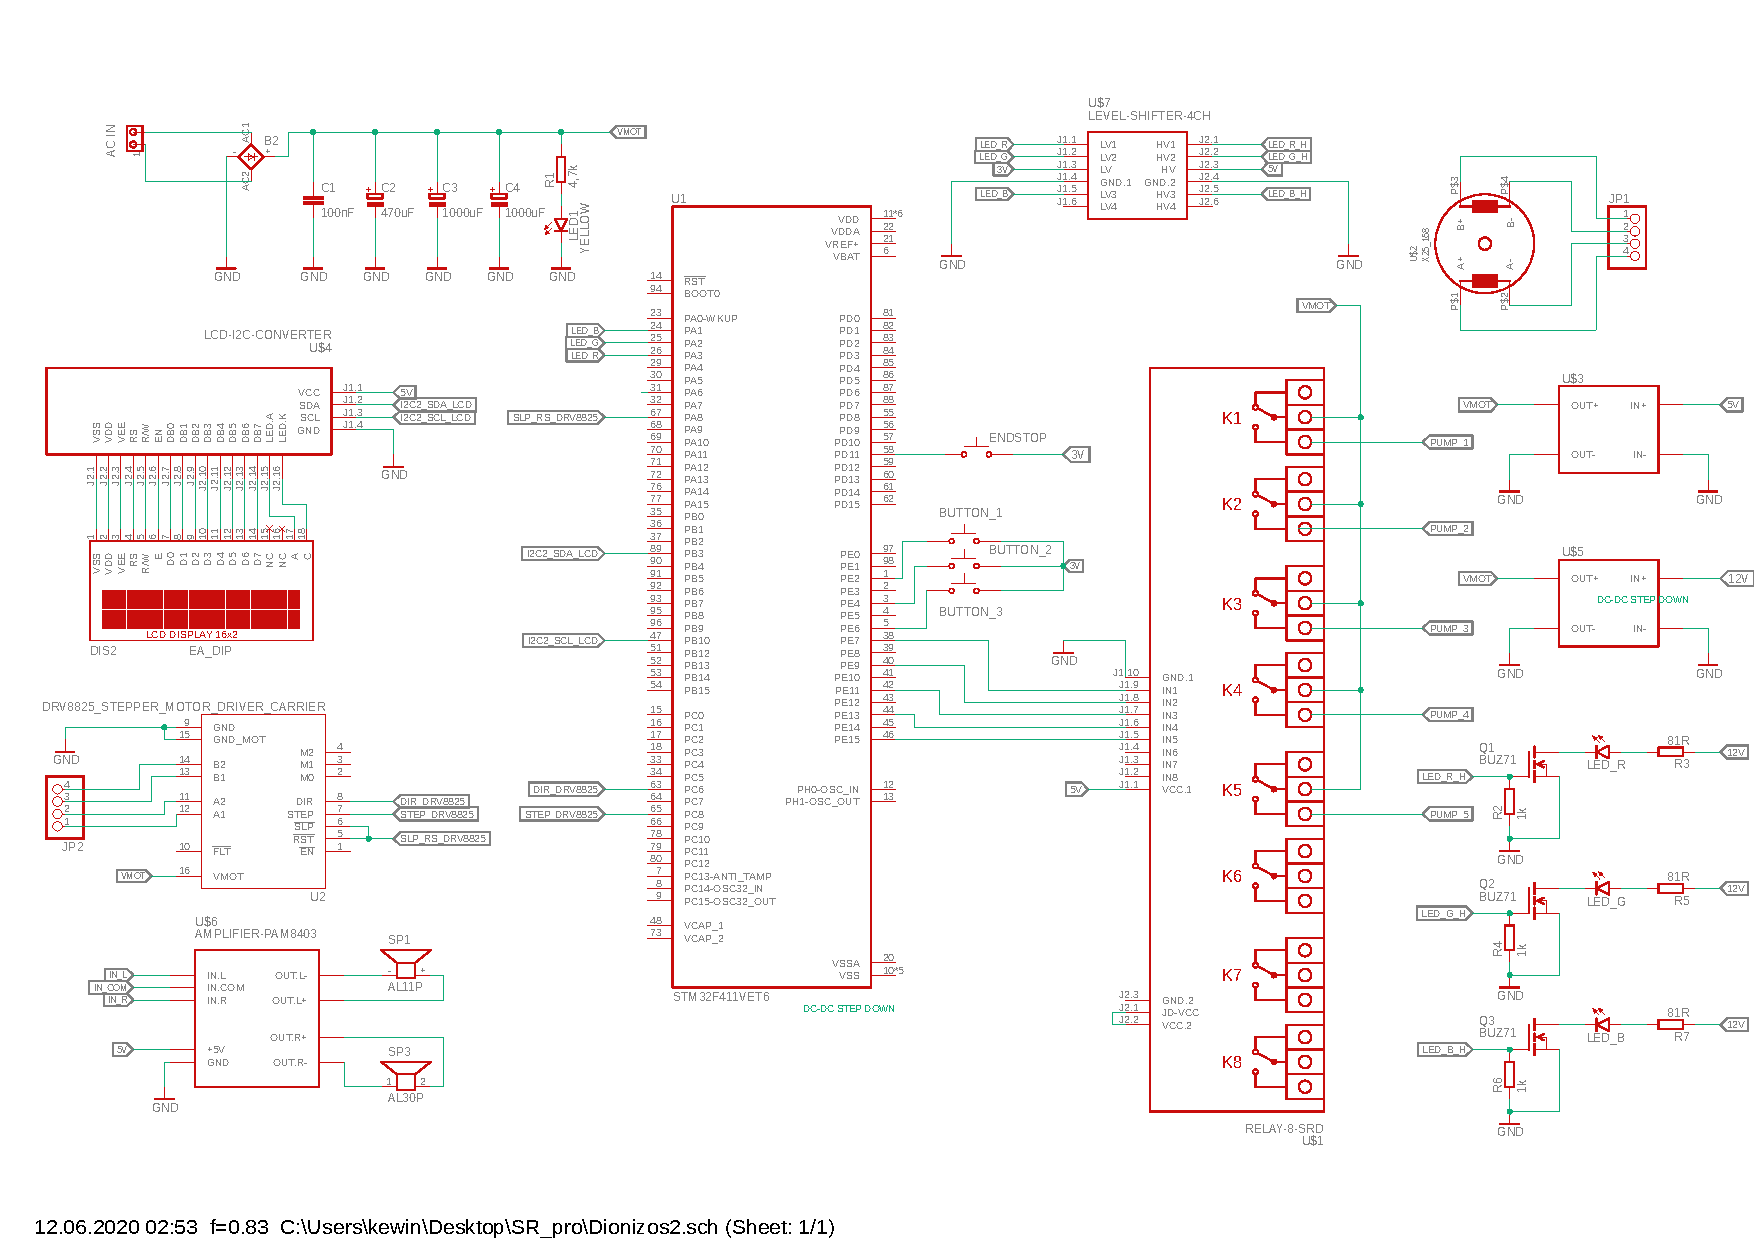
\includepdf[pages=-,pagecommand={},width=\textwidth,angle=90]{ajubadi2schemat.pdf}


%Obecne w dokumencie do etapu II oraz III
\section{Konstrukcja mechaniczna}

\subsection{Konstrukcja}
Jako podstawę do stworzenia urządzenia wykorzystano część mechaniki z drukarki HP C1440. Usunięto zbędne elementy wyposażenia, pozostawiono między innymi wałek, karetkę, Celem poprawienia estetyki projektu zmodyfikowano część podstawy przez montaż profili alumuniowych. W górnej części barmana umieszczona została aluminiowa listwa, pod którą przyklejona została taśma LED. Na niej w przyszłości również zostaną zamontowane wężyki prowadzące z pomp. 
Na jednym z profili umieszczono wyświetlacz LCD oraz przyciski sterujące. Na jego przedłużeniu znajduje się również sterownik całego urządzenia.

Jako podstawę użyto płyty laminowanej, którą wyposażono w gumowe nóżki. 

\subsection{Konserwacja}
Z uwagi na zużycie paska klinowego dokonano jego wymiany na nowy. Wyczyszczono wszystkie elementy ruchome urządzenia oraz użyto oleju do maszyn celem zmiejszenia oporów ruchu karetki po wałku. Dokonano również korekcji napięcia paska klinowego. 

\subsection{Zmiany w konstrukcji}
W drukarce do poruszania karetką wykorzystany był silnik prądu stałego, który został wymieniony na silnik krokowy. Z uwagi na różnicę w średnicach osi obu silników dokonano rozwiercenia zębatki, którą umieszczono na wale silnika krokowego. Do konstrukcji przykręcony został wyłącznik krańcowy.
Odcięto zbędne elementy plastikowe utrzymujące ruchome element.


\begin{figure}[H]
	\centering
	\includegraphics[width=0.7\textwidth]{sterownik.jpg}
	\caption{Wygląd całego urządzenia}
	\label{fig:Barman}
\end{figure}
\newpage


%Obecne w dokumencie do etapu II oraz III
\section{Opis działania programu}

Zaimplementowano obsługę silnika krokowego oraz wyłącznika krańcowego.

\begin{figure}[H]
	\centering
	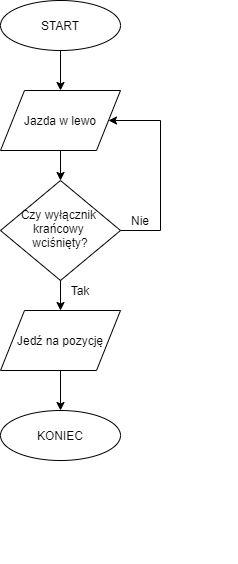
\includegraphics[width=0.35\textwidth]{algorytm2.png}
	\caption{Diagram algorytmu sterowania silnikiem}
	\label{fig:Diagram}
\end{figure}
 \newpage
 
Jednocześnie wykonywane są poszczególne elementy programu - obsługa przycisków i menu, odtwarzanie muzyki, obsługa silnika i przekaźników pomp oraz generowanie przebiegu PWM. Dzięki zastosowanym mechanizmom flag i zmiennych ulotnych oraz użyciu liczników niniejsze elementy mogą wykonywać się w tej samej chwili.
 
%Sekcję tą można podzielić na dodatkowe podsekcje w miarę potrzeb. 
%Do tego celu nalezy wykorzystać \textit{subsection}.
%
%W przypadku, dodania istotnego fragmentu kodu należy posłużyć się środowiskiem 
%lstlisting:
%
%\begin{lstlisting}[tabsize=2]
%int foo(void){
%return 2;
%}
%\end{lstlisting}
%
%Przykładowy wzór (\ref{eq:Wzor}):
%\begin{equation}
%\label{eq:Wzor}
%\Theta = \int_t^{t+dt} \omega \, dt.	
%\end{equation}
%
%Przykładowa pozycja bibliograficzna \cite{SR01} znajduje się 
%w pliku bibliografia.bib.

% %Obecne w dokumencie do etapu II oraz III (jeśli coś zostało niezrealizowane)
% \section{Zadania niezrealizowane}

% Jeśli wszystkie zadania zostały realizowane to wówczas 
% ta sekcja powinna być usunięta w całości. W przeciwnym razie
% należy zawrzeć tutaj, jakie zadania zostały nie zrealizowane 
% oraz jaka była tego przyczyna.

%Obecne we wszystkich dokumentach
\section{Podsumowanie}

Dokonano zmian w konfiguracji mikrokontrolera celem dopasowania rozmieszczenia pinów i uproszczenia połączeń na płytce uniwersalnej. Stworzono część mechaniczną i elektroniczną, która w razie potrzeb może zostać zmodyfikowana i dopasowana do rozwiązań, które nie zostały jeszcze użyte. Program obsługujący sterownik silnika krokowego z wykorzystaniem przerwań daje możliwość sterowania silnikiem i ustawienia rządanej pozycji, na której powinna znaleźć się karetka.


\newline
\newline
Linki do repozytoriów na platformie Github
\newline
\href{https://github.com/kewingaluszka/SteRoP_2020_AuBaDi_KGAU_2}{[Raport SteRoP\_2020\_AuBaDi\_KGAU\_2 - Github]}
\newline
\href{https://github.com/kewingaluszka/AuBaDi}{[Projekt STM32CubeIDE -- Github]}

\newpage
%\addcontentsline{toc}{section}{Bibilografia}
%\bibliography{bibliografia}
%\bibliographystyle{plabbrv}
\begin{thebibliography}{9}

\bibitem{stm}
    A. Kurczyk, \emph{Mikrokontrolery STM32 dla początkujących.}, Wydawnictwo Btc, Legionowo 2019
\bibitem{XD}
    A. France, \emph{Świat druku 3D. Przewodnik}, Wydawnictwo Helion, Gliwice 2014
\bibitem{polulu}
    Nota katalogowa A4988, \url{https://botland.com.pl/pl/index.php?controller=attachment&id_attachment=87}, 2009
\bibitem{LCD}
    Nota katalogowa PCF8574, \url{https://botland.com.pl/index.php?controller=attachment&id_attachment=210}, 1997
\bibitem{USB otg}
    Bartek, \emph{Kurs STM32 F4 – 11 – Komunikacja przez USB}, 9 sierpień 2016. Dostępne w Forbot: \url{https://forbot.pl/blog/kurs-stm32-f4-11-komunikacja-przez-usb-id13477}
\bibitem{USB flash}
    Wojtek, \emph{12 STM32F4 - CubeMx - USB podłączenie pendriva}, 26 luty 2017. Dostępne w Elektornika i Programowanie \url{https://elektronika327.blogspot.com/2017/02/12-stm32f4-cubemx-usb-podaczenie.html}
\bibitem{DAC}
    Nota aplikacyjna \emph{Audio and waveform generation using the DAC}, \url{https://www.st.com/resource/en/application_note/cd00259245-audio-and-waveform-generation-using-the-dac-in-stm32-microcontrollers-stmicroelectronics.pdf}, 2017
%\bibitem{Silnik skokowy Mineba 17PM}
%Silnik skokowy Mineba 17PM
%\url{http://cnc25.free.fr/documentation/moteurs}
%    Nota katalogowa Mineba 17PM-K, \url{https://www.eminebea.com/en/product/rotary/steppingmotor/hybrid/standard/__icsFiles/afieldfile/2017/09/29/17pm-k_1.pdf}
\bibitem{Audio playback and recording using the STM32F4DISCOVERY}
    Nota aplikacyjna \emph{Audio playback and recording},
    \url{https://www.st.com/resource/en/application_note/dm00040802-audio-playback-and-recording-using-the-stm32f4discovery-stmicroelectronics.pdf}, 2011
\bibitem{8 Channel 5V Optical Isolated Relay Module}
    Instrukcja obsługi modułu przekaźników, \url{http://www.handsontec.com/dataspecs/module/8Ch-relay.pdf}
\end{thebibliography}
\end{document}







































